% CHAPTER: WEC-Sim Structure                                                   %
% Included in documentation.tex, 3rd chapter 
% Author: Carlos :)
  	
\chapter{Library Structure} 
    \section{Library Structure Overview}
    The WEC-Sim library is divided into 4 sublibraries. The user
    should be able to model their WEC device using the available WEC-Sim blocks, 
	and possibly some \simmechanics blocks. Table \ref{tab:libStruct} lists the WEC-Sim 
	blocks and their organization into sublibraries.
	
        % Table generated by Excel2LaTeX
         \begin{table}[htbp]
          \centering
          \caption{WEC-Sim library structure}
            \begin{tabular}{c|c}
            \toprule
            \multicolumn{2}{c}{\textbf{WEC-Sim Library}} \\
            \midrule
            \textbf{Sublibrary} & \textbf{Blocks} \\
            \midrule
            \multirow{1}[2]{*}{\texttt{Body Elements}} & \texttt{Rigid Body} \\
            \midrule
            \multirow{1}[2]{*}{\texttt{Frames}} & \texttt{Global Reference 
			Frame} \\
            \midrule
            \multirow{5}[2]{*}{\texttt{Constraints}} & Heave \\
                  & \texttt{Pitch} \\
                  & \texttt{Surge} \\
                  & \texttt{Fixed} \\
                  & \texttt{Floating} \\
            \midrule
            \multirow{3}[2]{*}{\texttt{PTOs}} & \texttt{Rotational PTO 
			(Local RY)} \\
                  & \texttt{Translational PTO (Local X)} \\
                  & \texttt{Translational PTO (Local Z)} \\
            \bottomrule
            \end{tabular}
          \label{tab:libStruct}
        \end{table}
		
    In the following sections, we will describe the four sublibraries and their general purpose.
    The \texttt{Body Elements} sublibrary contains the \texttt{Rigid Body} block 
    used to simulate the different bodies. The \texttt{Frames} sublibrary contains the 
    \texttt{Global Reference Frame} block necessary for every simulation. The \texttt{Constraints} 
    sublibrary contains blocks that are used to constrain the DOF of the bodies, without including 
    any additional forcing or resistance. The \texttt{PTOs} sublibrary contains blocks used to both 
    simulate a PTO system and restrict the body motion. Both constraints and PTOs can be used 
    to restrict the relative motion between multibody systems.
    %\end{section}{Library Structure Overview}
 
    \section{\texttt{Body Elements} Sublibrary}
    The \texttt{Body Elements} sublibrary (Figure~\ref{fig:bLib}) 
    contains one block, \texttt{Rigid Body} block. It is used to 
    represent rigid bodies. At least one instance of this block is required in 
    each model.
	
    \begin{figure}[H]        
    \centering        
    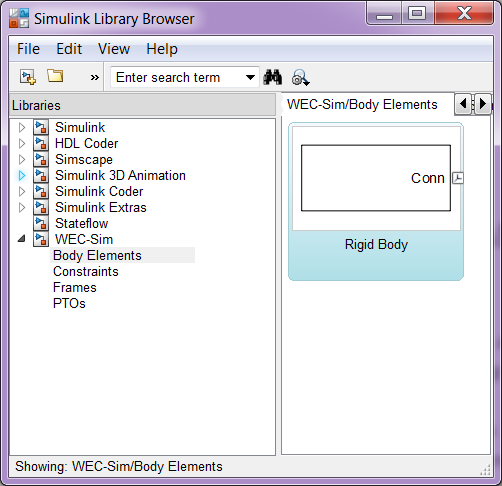
\includegraphics[width=0.6\textwidth]{libraryStructure/figures/bodiesLib}        
    \caption{\texttt{Body Elements} sublibrary}        
    \label{fig:bLib}        
    \end{figure}

        \subsection{\texttt{Rigid Body} Block}
        The \texttt{Rigid Body} block is used to represent a rigid body in the 
		simulation.
		The user has to name the blocks 'body(i)' where i=1,2,\ldots. 
		The mass properties, hydrodynamic data, geometry file, mooring, and 
		other properties are then specified in the input file. Within the body 
		block the wave radiation, wave excitation, hydrostatic restoring, viscous damping and mooring forces are calculated.
    %\end{subsection}{\texttt{Rigid Body} Block}
    %\end{section}{\texttt{Body Elements} Sublibrary}  

    \section{\texttt{Frames} Sublibrary}
    The \texttt{Frames} sublibrary, shown in Figure~\ref{fig:fLib}, contains one block 
    that is necessary in every model. The \texttt{Global Reference Frame} block defines global references 
    and can be thought of as the seabed.
    
        \subsection{\texttt{Global Reference Frame} Block}
		The \texttt{Global Reference Frame} block defines the solver 
		configuration, seabed 
		and free surface description, simulation time, and other global 
		settings. It can be useful to think of the \texttt{Global Reference Frame}
		as being the seabed when creating a model. 
		Every model requires one instance of the \texttt{Global 
		Reference Frame}
		block. The \texttt{Global Reference Frame} block uses the simulation 
		class variable \texttt{simu} and the wave class variable \texttt{waves},
		which must be defined in the input file.
		
		\begin{figure}[H]        
		\centering
		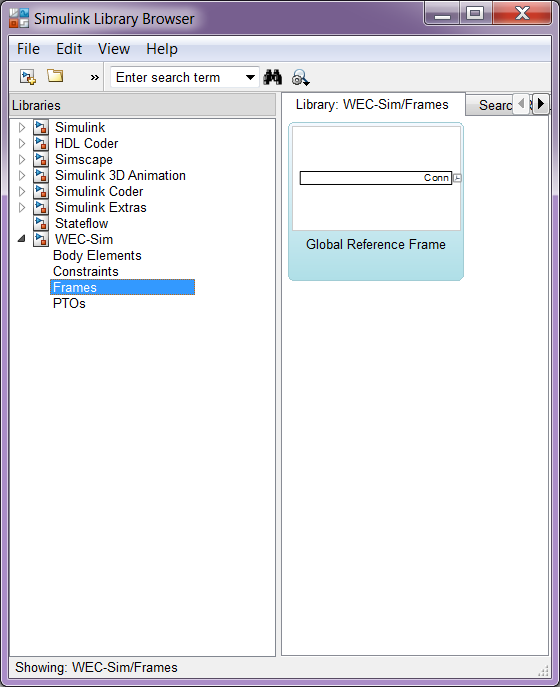
\includegraphics[width=0.6\textwidth]{libraryStructure/figures/framesLib}
		\caption{\texttt{Frames} sublibrary}
		\label{fig:fLib}
		\end{figure}	
    
         %\end{subsection}{\texttt{Global Reference Frame} Block}
    %\end{section}{\texttt{Frames} Sublibrary}

    \section{\texttt{Constraints} Sublibrary}
    The blocks within the \texttt{Constraints} sublibrary, shown in Figure~\ref{fig:cLib}, are used to 
    define the DOF of a specific body. \texttt{Constraints} blocks define only the DOF, but do not 
    otherwise apply any forcing or resistance to the body motion. Each \texttt{Constraints} block 
    has two connections, a base (B) and a follower (F). The \texttt{Constraints} block restricts the 
    motion of the block that is connected to the follower relative to the block that is connected to the base. 
    The base of these blocks is typically the \texttt{Global Reference Frame} (which can be thought of as 
    the seabed) and the follower is a \texttt{Rigid Body}. 
			  
    There are five \texttt{Constraints} blocks, including three that restrict motion to one 
	DOF (\texttt{Heave}, \texttt{Surge}, \texttt{Pitch}), a free-floating (\texttt{Floating}) 
	block, and a rigid connection (\texttt{Fixed}) block. 
	The rest of this section will describe each \texttt{Constraints} block in more detail.

	\begin{figure}[H]        
	\centering        
	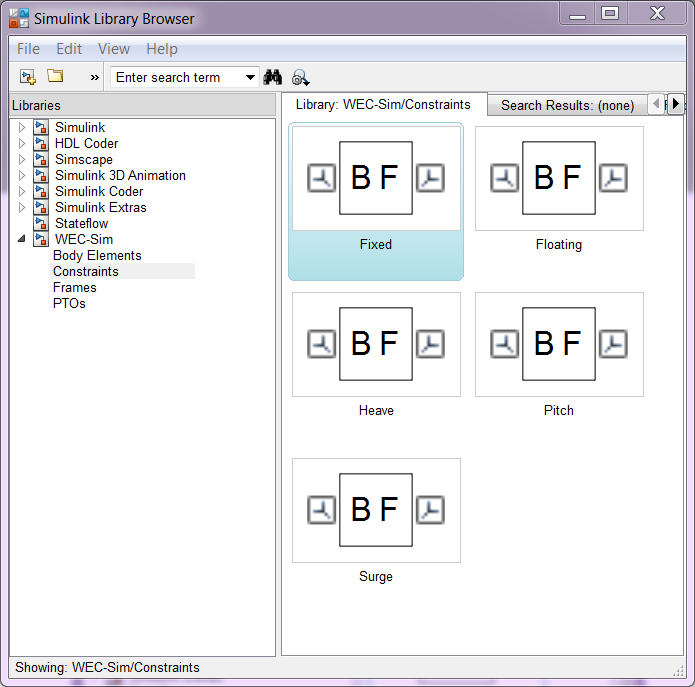
\includegraphics[width=0.6\textwidth]{libraryStructure/figures/constraintsLib}        
	\caption{\texttt{Constraints} sublibrary}        
	\label{fig:cLib}        
	\end{figure}
	
        \subsection{\texttt{Floating} Block}
        The \texttt{Floating} block is used to simulate a free-floating body. It
		constrains the motion of the follower to be along the XZ plane of 
		the base. That is, it allows translation in the X- and 
		Z-axis, and rotation about the Y-axis. It  is usually used with the base 
		connected to the \texttt{Global Reference Frame} (seabed), in which 
		case the motion of the follower is along the global XZ plane. 
        %\end{subsection}{3DOF SurgeHeavePitch Block}

        \subsection{\texttt{Heave} Block}
        The \texttt{Heave} block constrains the motion of the follower
        relative to the base to be along the Z-axis. 
        In the case of the base connected to the \texttt{Global Reference 
		Frame} (seabed), the body is allowed to
        move only in the vertical (Z) direction. In the case of the \texttt{Heave} 
        block connecting two bodies, the relative motion of the two 
        bodies is constrained
        to be only along their Z-axes. 
        The Z-axis of the follower
        and base will always be parallel and their perpendicular distance will
        be constant. The actual direction of movement of the follower depends on
		the orientation of the base.
        %\end{subsection}{1DOF Heave Block}

		\subsection{\texttt{Surge} Block}
        The \texttt{Surge} block constrains the motion of the follower
        relative to the base to be along the X-axis. If the base is connected to 
        the \texttt{Global Reference Frame} (seabed), the body is allowed to
        move only in the horizontal (X) direction. If \texttt{Surge} 
        block is connects two bodies, the relative motion of the two 
        bodies is constrained to be only along their X-axes. The X-axis of the follower
        and base will always be parallel and their perpendicular distance will
        be constant. The actual direction of movement of the follower depends on 
        the orientation of the base.
        %\end{subsection}{\texttt{Surge} Block}


        \subsection{\texttt{Pitch} Block}
        The \texttt{Pitch} block constrains the relative motion between the 
        follower and the base to be pitch rotation only (about the Y-axis). The 
        distance from both body-fixed coordinate systems to the point of rotation
        stays constant. The orientation of both body-fixed Y-axes also stays
        constant. The user MUST enter the point about which the rotation occurs 
        as the constraint's location in the input file. 
        %\end{subsection}{\texttt{Pitch} Block}

        \subsection{\texttt{Fixed} Block}
        The \texttt{Fixed} block is a rigid connection that constrains all 
        motion between the base and follower. It restricts translation in the X- and Z-axis, 
        and rotation about the Y-axis.  Its most common use is for a rigid body  
        fixed to the seabed. 
        %\end{subsection}{\texttt{Fixed} Block}
    %\end{section}{\texttt{Constraints} Sublibrary}
	
    \section{\texttt{PTOs} Sublibrary}
	The \texttt{PTOs} sublibrary, shown in Figure~\ref{fig:pLib}, is used to 
	simulate simple PTO systems and to restrict relative motion between multiple 
	bodies or between one body and the seabed. The \texttt{PTO} blocks can simulate 
	simple PTO systems by applying a linear stiffness and damping to the connection. 
	Similar to the \texttt{Constraints} blocks, the \texttt{PTO} blocks have a base (B) 
	and a follower (F). Users MUST name each \texttt{PTO} block 'pto(i)' where i=1,2,
	\ldots, and then define their properties in the input file.
	
        \subsection{Translation PTO (Local Z) Block}
        The \texttt{Translation PTO (Local Z)} is identical to the 
		\texttt{Heave} constraint, but applies a linear stiffness and 
		damping coefficient to the connection. The user has to name the PTOs as 
		described earlier. The user then specifies the stiffness coefficient (in N/m), and 
		damping coefficient (in Ns/m) in the input file.
        %\end{subsection}{Heave Joint (Translation) Block}
	\begin{figure}[H]        
	\centering        
	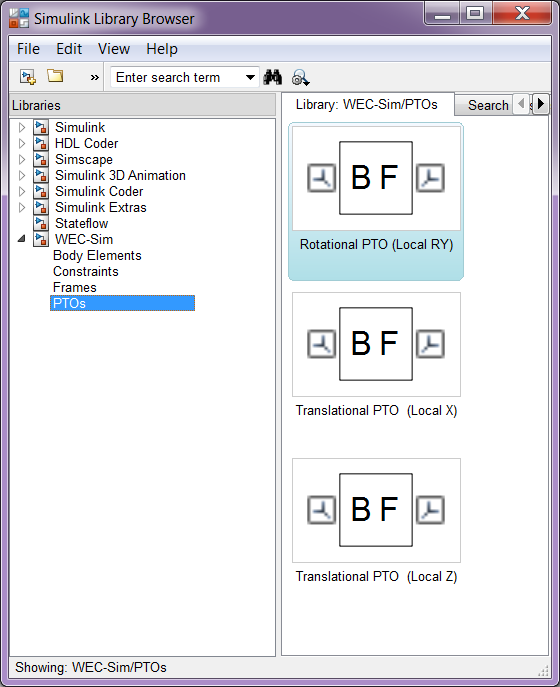
\includegraphics[width=0.6\textwidth]{libraryStructure/figures/ptosLib}        
	\caption{\texttt{PTOs} sublibrary}        
	\label{fig:pLib}        
	\end{figure}
	
        \subsection{Translation PTO (Local X) Block}
        %\FloatBarrier
        The \texttt{Translation PTO (Local X)} is identical to the 
		\texttt{Surge} constraint, but additionally applies a linear stiffness 
		and damping coefficient to the connection. The user has to name the PTOs as 
		described earlier. The user then specifies the stiffness coefficient (in N/m), and 
		damping coefficient (in Ns/m) in the input file.
        %\end{subsection}{Heave Joint (Translation) Block}
	        
        \subsection{Rotational PTO (Local RY) Block}
        %\FloatBarrier
        The \texttt{Rotational PTO (Local RY)} is identical to the \texttt{Pitch} constraint, 
                     but adds a linear rotational stiffness and damping coefficient to the connection. 
                     The user has to name the PTOs as described earlier. The user then specifies 
                     the stiffness coefficient (in Nm/rad) and damping coefficient (in Nms/rad) in the input file.
        %\end{subsection}{Pitch Joint (Rotation) Block}
    %\end{section:Joint Blocks}

		
    \section{Other SimMechanics Blocks}
    %\FloatBarrier
    In some situations, users may have to use \simmechanics blocks not included in
    the WEC-Sim Library to build their WEC model. One commonly used block is the \texttt{Rigid Transform}, 
    which can be used to rotate the frames on PTOs,cconstraints, and bodies. 
    This is also explained in the \simmechanics {User's Guide} \cite{simMechanics2014}.
      %\end{section:A Note on \simmechanics, Coordinate Systems,and Constraint Direction}  
%\end{chapter:WEC-Sim Library Structure}
